\chapter{Character}

	\section{Introduction}
		Each character extends the Character class. The \emph{update} method must be implemented. 
		
		
		
	Each Character consists of a set of actions.
	
	To create an character, must firstly create actions, then add the actions to character. After this, the method \textbf{String buildCharacter()} must be called in order to check and create character actions dependecy.
	
	Each Action have its dependencies, in other words, to create an Action you need to create all Actions necessary to this Action. All these actions are added to the character.
	
	\section{File Format}
	\begin{algorithm}[H]
	    \caption{Character description File Format.}
	    \label{algoEvalCuda}
	    \begin{algorithmic}
			\STATE CREATE\_DIR
			\STATE [F][STRING] CLASS\_NAME
			\STATE [F][STRING]CHAR\_NAME
			\FOR {EACH ACTION}
				\STATE WRITE\_ACTION\_INSIDE\_DIR
				\STATE [F][STRING]ACTION\_NAME
			\ENDFOR
			%\STATE [F][STRING] NUMBER\_OF\_BUTTON\_MAPS
			%\FOR {EACH BUTTON\_MAP}
			%	\STATE [F][INT] KEY\_CODE
			%	\STATE [F][STRING] ACTION\_NAME
			%\ENDFOR
		\end{algorithmic}
	\end{algorithm}
	
	\section{Collision Types}
	\begin{table}[H]
    \caption{Possible collisions with the scenary.}
    \label{tab:scenaryCollisionTypes}
    \centering
	
    \begin{tabular}{|l|c|}
		\hline
		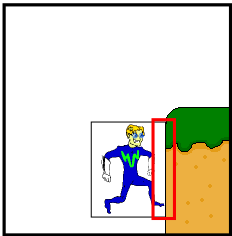
\includegraphics[width = 3cm]{img/leftright_collision.png} & COLLISION\_SCENARY\_LEFT\_RIGHT \\
		\hline
		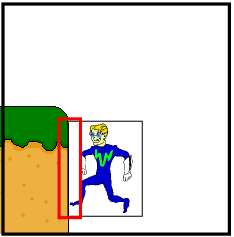
\includegraphics[width = 3cm]{img/rightleft_collision.png} & COLLISION\_SCENARY\_RIGHT\_LEFT \\
		\hline
		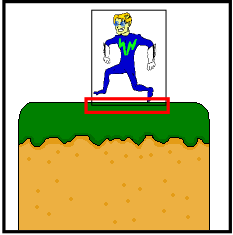
\includegraphics[width = 3cm]{img/updown_collision.png} & COLLISION\_SCENARY\_UP\_DOWN \\
		\hline
		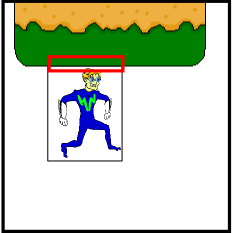
\includegraphics[width = 3cm]{img/downup_collision.png} & COLLISION\_SCENARY\_DOWN\_UP \\
		\hline
		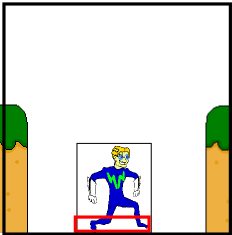
\includegraphics[width = 3cm]{img/outscenary_collision.png} & COLLISION\_SCENARY\_OUT\_SCENARY \\
		\hline
	\end{tabular}
	\end{table}
	
	\section{The Update Method}
	The update method must be implemented in the subclass.  It's the most important method, wich will determine all characters caracterstics.
	
	Fisrtly, analise inputs in the Joypad.buttonBuffer. For each button pressed verifies if can activate the associated action (by the ACTIVATION\_KEY). 